\chapter{Message Passing Interface}

The Message Passing Interface (MPI) is a standardized library that implements the distributed memory programming model. Its primary purpose is to facilitate data movement between distinct address spaces in a parallel computing environment.

In MPI, each process operates as an independent entity with its own private memory space. From a programming perspective, memory management within each process follows the same principles as sequential programming, making it conceptually straightforward for developers.

Processes interact through explicit message passing for both synchronization and data exchange. This communication model requires explicit collaboration between processes - data is only shared when processes explicitly send and receive messages.

It's important to note that MPI is implemented as a library rather than a programming language. This means that all parallel operations are performed through library function calls, which provides flexibility in terms of language integration while maintaining a consistent interface across different platforms.

So here must exist a way to send a message from one process to another; this method should accept the following parameters:

\begin{itemize}
    \item the message to send
    \item the length of the message
    \item the receiver process
    \item the framework this message belongs to
\end{itemize}

In the same way, there must be a way to receive a message from another process; this method should accept the following parameters:
\begin{itemize}
    \item where to store the message
    \item the length of the message
    \item the sender process
    \item the framework this message belongs to
\end{itemize}

So, we expect that there must be point-to-point
\begin{itemize}
    \item a way to send messages
    \item a corresponding way to receive messages
    \item a way to know “the names” in “the framework”
\end{itemize}

Since sometimes we need to broadcast messages, it would be nice if:
\begin{itemize}
    \item there was a broadcasting (one-to-many) mechanism
    \item there was a collection mechanism (many-to-one) mechanism
    \item the answer/collection was possible many-to-many
\end{itemize}

\subsubsection{Communicators}

Communicators and groups are a very central concepts in MPI: tasks can form groups (a task can belong to more than one group) and the same group can be in different situations.

The \bfit{communicator} is the combination of a group and its “context”.

You can build as many groups as you want, and they may or not have a communicator. However, if you want to communicate among tasks in a group, you need a communicator.

This functionality offers the capability of isolating communication between application modules with an effective “sandbox” for different contexts.

For instance, a parallel library and your application will use internally their own communicator, separating contexts.

\begin{itemize}
    \item By creating groups of MPI processes, that may or not overlap with each other, it is possible to
    \begin{itemize}
        \item separate contexts within different modules of the same application
        (useful or even advisable)
        \item express multiple levels of parallelism
    \end{itemize}
\end{itemize}

MPI provides several predefined communicators that are available after initialization:

\begin{itemize}
    \item \texttt{MPI\_COMM\_WORLD} is the default communicator available right after the call to \texttt{MPI\_Init}. Its group contains all the tasks started by your job.
    
    \item \texttt{MPI\_COMM\_NULL} signals an invalid or non-existent communicator. This is often used as a return value to indicate errors in communicator operations.
    
    \item \texttt{MPI\_COMM\_SELF} contains only the process itself. This is useful when a process needs to communicate with itself.
    
    \item \texttt{MPI\_GROUP\_NULL} signals an invalid or non-existent group. Similar to \texttt{MPI\_COMM\_NULL}, it's used to indicate errors in group operations.
\end{itemize}

These predefined communicators serve as fundamental building blocks for MPI communication patterns and are essential for both basic and advanced MPI programming.

\subsubsection{Send and Receive}

MPI provides two basic functions for sending and receiving messages between processes:

\begin{codeblock}[language=C]
int MPI_Send(
    const void *buf,        /* starting address of send buffer */
    int count,              /* number of elements in send buffer */
    MPI_Datatype datatype,  /* datatype of each buffer element */
    int dest,               /* rank of destination */
    int tag,                /* message tag */
    MPI_Comm comm           /* communicator */
)
\end{codeblock}

\begin{codeblock}[language=C]
int MPI_Recv(
    void *buf,              /* starting address of receive buffer */
    int count,              /* number of elements in receive buffer */
    MPI_Datatype datatype,  /* datatype of each buffer element */
    int source,             /* rank of source */
    int tag,                /* message tag */
    MPI_Comm comm,          /* communicator */
    MPI_Status *status      /* status object */
)
\end{codeblock}

The data type is a fundamental concept in MPI. It defines the type of data being sent or received. MPI provides a variety of predefined data types, including:

\begin{table}[H]
    \centering
    \begin{tabular}{|l|l|}
        \hline
        \textbf{MPI DataType} & \textbf{C DataType} \\
        \hline
        \plaintt{MPI\_CHAR} & \plaintt{char} \\
        \plaintt{MPI\_BYTE} & \plaintt{unsigned char} \\
        \plaintt{MPI\_SHORT}, \plaintt{MPI\_UNSIGNED\_SHORT} & (\plaintt{unsigned}) \plaintt{short int} \\
        \plaintt{MPI\_INT}, \plaintt{MPI\_UNSIGNED\_INT} & (\plaintt{unsigned}) \plaintt{int} \\
        \plaintt{MPI\_LONG}, \plaintt{MPI\_UNSIGNED\_LONG} & (\plaintt{unsigned}) \plaintt{long int} \\
        \plaintt{MPI\_LONG\_LONG}, \plaintt{MPI\_UNSIGNED\_LONG\_LONG} & (\plaintt{unsigned}) \plaintt{long long int} \\
        \plaintt{MPI\_FLOAT} & \plaintt{float} \\
        \plaintt{MPI\_DOUBLE} & \plaintt{double} \\
        \plaintt{MPI\_LONG\_DOUBLE} & \plaintt{long double} \\
        \plaintt{MPI\_PACKED} & \plaintt{--} \\
        \hline
    \end{tabular}
    \caption{Correspondence between MPI predefined datatypes and C datatypes.}
    \label{tab:mpi-c-datatypes}
\end{table}

\begin{exampleblock}[Send and Receive Example]
    \begin{codeblock}[language=C]
int N;
if ( Myrank == 0 )
    MPI_Send( &N, 1, MPI_INT, 1, 0, MPI_COMM_WORLD );
else if ( Myrank == 1 ) {
    MPI_Status status;
    MPI_Recv( &N, 1, MPI_INT, 0, 0, MPI_COMM_WORLD, &status );
}
else if ( Myrank == 1 )
    MPI_Recv( &N, 1, MPI_INT, 0, 0, MPI_COMM_WORLD, MPI_STATUS_IGNORE );
    \end{codeblock}

    \underline{\textbf{NOTE}}: \plaintt{MPI\_STATUS\_IGNORE} is always valid instead of putting an \plaintt{MPI\_Status} varible's address as last argument of \plaintt{MPI\_Recv}
\end{exampleblock}

\begin{exampleblock}[Sending things of different types]
    \begin{codeblock}[language=C]
typedef struct {
    int i, j;
    double d, f;
    char s[4];
} my_data;

unsigned int length = N * sizeof(my_data);

if (Myrank == 0) {
    MPI_Send(data, length, MPI_BYTE, 1, 0, MPI_COMM_WORLD);
} else if (Myrank == 1) {
    MPI_Recv(data, length, MPI_BYTE, 0, 0, MPI_COMM_WORLD,
             MPI_STATUS_IGNORE);
}
    \end{codeblock}
\end{exampleblock}

\dots

\missing{probe}

\dots

When we do send a message, we specify the memory region that contains the data, at what point in the future it is safe to modify the memory region involved in the send? Or better, how can we be sure that the communication has ended and the data have all been received?

The MPI standard prescribes that \plaintt{MPI\_Send} returns when it is safe to modify the send buffer. So, whenever \plaintt{MPI\_Send} returns, it is safe to act on the memory region that has been sent.

\dots

\missing{protocols}

\dots

Code that rely on the system's bufferization to run correctly are called \bfit{unsafe}.

Solution to cure, or better, to avoid the unsafe situations are:

\begin{itemize}
    \item designing more carefully the communication pattern
    \item checking the runnability by substituting \plaintt{MPI\_Send} with \plaintt{MPI\_Ssend}
    \item using \plaintt{MPI\_Sendrecv}
    \item supplying explicitly buffer with \plaintt{MPI\_Bsend}
    \item non-blovking operations
\end{itemize}

\begin{figure}[H]
    \centering
    \includegraphics[width=0.5\textwidth]{assets/unsafe-code.png}
    \caption{Deadlock, Unsafe and Safe code}
    \label{fig:unsafe-code}
\end{figure}

\missing{boh}

There are different routines to send and receive messages:

\begin{table}[H]
    \centering
    \begin{tabular}{|p{3cm}|l|p{10cm}|}
        \hline
        \textbf{mode} & \textbf{routine} & \textbf{notes} \\
        \hline
        \hline
        standard & \plaintt{MPI\_Send} & Safe to modify data once returns. Equiv. to synchronous or asynchronous mode (uses sys buffers) depending on msg size and implementation choices. \\
        \hline
        synchronous & \plaintt{MPI\_Ssend} & Completes when the receive has started (it does not wait for the receive completion). Unsafe communication patterns will deadlock $\rightarrow$ a way to check safety. \\
        \hline
        asynchronous or "buffered" & \plaintt{MPI\_Bsend} & Completes after the buffer has been copied. Needs an explicit buffer. \\
        \hline
        ready & \plaintt{MPI\_Rsend} & Mandatory that the matching receive has already been posted. May be the fastest solution, but it is quite problematic. \\
        \hline
        all & \plaintt{MPI\_Recv} & One size serves 'em all \\
        \hline
    \end{tabular}
    \caption{Different MPI send and receive routines}
    \label{tab:mpi-routines}
\end{table}

\missing{examples}

\subsubsection{Non-Blocking communications}

Until now we have considered point-to-point communication functions that do not return until some conditions are met (either the copy of the data into a buffer or the actual delivery of the data to the recipient, in case of the sender, or the actual arrival of the data into their local destination in case of the receiver).

As such, the caller is blocked into the call and cannot perform any other operation. Those functions are consequently identified as \bfit{blocking functions}.

If what follows the Send/Recv depends on the fact that the operations mentioned above actually completed, then the usage of those functions reflects an actual dependency and there is little to be done.

However, if there are other instructions that could be executed while waiting for the data to arrive at destination, by using blocking functions we are losing parallelism.

To obviate to this issue, MPI offers the non-blocking functions, i.e. a set of functions that return immediately.

However, their return does not mean that the communication has completed but only that it has been posted on an internal queue system that will execute it at some point in the future.

To assess, at any moment, whether the communication has been executed, MPI provides dedicated routines:

\begin{codeblock}[language=C]
MPI_Test ( MPI_Request *, int *flag, MPI_Status *)
MPI_Wait ( MPI_Request *, MPI_Status *)
MPI_Waitall (int count, MPI_Request array_of_req[], MPI_Status array_of_st[] )
\end{codeblock}

The non-blocking counterparts of the send and receive functions are:

\begin{codeblock}[language=C]
int MPI_Isend( void *buf, int count, MPI_Datatype dtype,
               int dest, int tag, MPI_Comm comm,
               MPI_Request *request );

int MPI_Irecv( void *buf, int count, MPI_Datatype datatype,
               int source, int tag, MPI_Comm comm,
               MPI_Request *request );
\end{codeblock}

The request variable is used to handle the status of the \plaintt{MPI\_Isend} or \plaintt{MPI\_Irecv} operation posted. At any point after the call, the status can be determined by the immediately-returning call

\begin{tipsblock}[Non-blocking communication pattern]
    When using non-blocking communication, always follow this three-step pattern: 
    
    \begin{enumerate}
        \item \textbf{Post the operation}: Call \plaintt{MPI\_Isend} or \plaintt{MPI\_Irecv} to initiate the communication. This returns immediately with a request handle.
        
        \item \textbf{Overlap computation}: Perform other useful work while the communication proceeds asynchronously in the background. This is where the performance benefit comes from.
        
        \item \textbf{Ensure completion}: Use \plaintt{MPI\_Wait} (blocking) or \plaintt{MPI\_Test} (non-blocking check) to verify the operation has finished before accessing the communicated data.
    \end{enumerate}
\end{tipsblock}
    
\begin{warningblock}[Critical safety rule]
    Never access the send buffer (for sends) or receive buffer (for receives) until the operation is confirmed complete via \plaintt{MPI\_Wait} or a successful \plaintt{MPI\_Test}. Violating this rule can lead to race conditions, data corruption, and undefined behavior.
\end{warningblock}

\dots

All the sending routines have a correspondent non-blocking version:

\begin{table}[H]
    \centering
    \begin{tabular}{|l|l|l|}
        \hline
        \textbf{mode} & \textbf{Blocking routine} & \textbf{Non-blocking routine} \\
        \hline
        standard & \plaintt{MPI\_Send} & \plaintt{MPI\_Isend} \\
        \hline
        synchronous & \plaintt{MPI\_Ssend} & \plaintt{MPI\_Issend} \\
        \hline
        asynchronous or "buffered" & \plaintt{MPI\_Bsend} & \plaintt{MPI\_Ibsend} \\
        \hline
        ready & \plaintt{MPI\_Rsend} & \plaintt{MPI\_Irsend} \\
        \hline
        \textit{all} & \plaintt{MPI\_Recv} & \plaintt{MPI\_Irecv} \\
        \hline
    \end{tabular}
    \caption{Comparison of blocking and non-blocking MPI communication routines}
    \label{tab:mpi-blocking-nonblocking}
\end{table}

\dots

\missing{boh}

\subsection{Collective operations}

Collective communication operations in MPI are fundamental for coordinating tasks and exchanging data among multiple processes simultaneously. These operations always occur within a specific group of processes defined by a communicator.

Key characteristics of collective communications include:
\begin{itemize}
    \item \textbf{Group-wide participation}: All processes within the communicator's group must participate in the collective operation. If even one process in the group does not call the collective function, the program will likely hang or behave unpredictably.
    \item \textbf{Implicit synchronization}: Collective operations often imply a synchronization point. Processes may block until all participating processes have reached the collective call. This synchronization can lead to some degree of serialization, potentially impacting overall parallelism.
    \item \textbf{Optimized algorithms}: MPI implementations typically use sophisticated and highly optimized algorithms for collective operations to ensure efficiency across various network topologies and system architectures.
    \item \textbf{Blocking and non-blocking variants}: Similar to point-to-point communication, many collective operations have both blocking and non-blocking versions (e.g., \plaintt{MPI\_Bcast} and \plaintt{MPI\_Ibcast}). Non-blocking collectives allow for potential overlap of computation and communication.
\end{itemize}

Collective operations can be broadly categorized into three main classes:

\begin{enumerate}
    \item \textbf{Synchronization}: These operations are used to synchronize processes within a group. The most common example is \plaintt{MPI\_Barrier}, which blocks each process until all processes in the communicator have called it.
    \item \textbf{Data Movement}: These operations involve distributing, gathering, or re-arranging data among processes.
    \item \textbf{Collective Computation (Reductions)}: These operations perform a computation (e.g., sum, max, min, logical AND) across data provided by all processes in the communicator, with the result being available at one (e.g., \plaintt{MPI\_Reduce}) or all (e.g., \plaintt{MPI\_Allreduce}) processes.
\end{enumerate}

We will now discuss the most common collective operations.

\subsubsection{Synchronization}

The \plaintt{MPI\_Barrier} function is a collective synchronization operation. Its primary purpose is to ensure that all processes within a specified communicator reach a certain point in their execution before any of them proceed further.

The function call \plaintt{int MPI\_Barrier(MPI\_Comm comm)} takes a communicator \plaintt{comm} as an argument. A process calling \plaintt{MPI\_Barrier} will block until all other processes in the group associated with \plaintt{comm} have also called this function. Once all processes have reached the barrier, they are all unblocked and can continue execution. While \plaintt{MPI\_Barrier} is useful for synchronizing tasks, it should be used judiciously.

Like any synchronization mechanism, it can introduce serialization into the parallel execution, potentially limiting performance gains by forcing faster processes to wait for slower ones.

\subsubsection{Collective data movement}

\begin{figure}[H]
    \centering
    \includegraphics[width=0.7\textwidth]{assets/data-movement.png}
    \caption{Data movement operations}
    \label{fig:data-movement}
\end{figure}

\begin{itemize}
\item \textbf{Broadcast:} The \plaintt{MPI\_Bcast} function is one of the most fundamental collective operations in MPI. It allows a single process (the root) to send the same data to all other processes in the communicator. The root process (P0) holds the data (A) and broadcasts it to all other processes. After the broadcast, all processes have a copy of the data.

\begin{figure}[H]
    \centering
    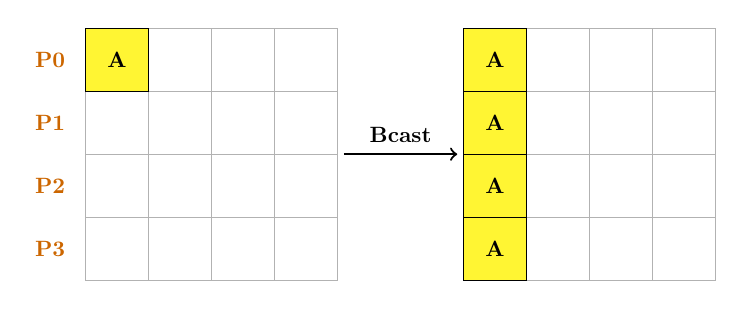
\begin{tikzpicture}[scale=0.8, every node/.style={scale=0.8}]
        %! --- Bcast ---
        % Process labels (left)
        \foreach \i/\p in {0/P0,1/P1,2/P2,3/P3} {
            \node[anchor=east] at (-0.2,3.5-\i) {\textcolor{orange!80!black}{\textbf{\p}}};
        }
        % Bcast left matrix
        \foreach \i in {0,...,3} {
            \foreach \j in {0,...,3} {
                \draw[gray!60] (0+\j,3-\i) rectangle (1+\j,4-\i);
            }
        }
        \node[fill=yellow!80,draw,minimum width=1cm,minimum height=1cm] at (0.5,3.5) {\textbf{A}};
        % Bcast right matrix
        \foreach \i in {0,...,3} {
            \foreach \j in {0,...,3} {
                \draw[gray!60] (6+\j,3-\i) rectangle (7+\j,4-\i);
            }
            \node[fill=yellow!80,draw,minimum width=1cm,minimum height=1cm] at (6.5,3.5-\i) {\textbf{A}};
        }
        % Bcast arrow and label
        \draw[->,thick] (4.1,2) -- (5.9,2);
        \node at (5,2.3) {\textbf{Bcast}};
    \end{tikzpicture}
    % \caption{Broadcast}
    \label{fig:bcast}
\end{figure}

\item \textbf{Scatter and Gather:} The \plaintt{MPI\_Scatter} and \plaintt{MPI\_Gather} functions are complementary collective operations that distribute and collect data among processes. \plaintt{MPI\_Scatter} takes data from a single process (the root) and distributes it among all processes, while \plaintt{MPI\_Gather} does the opposite - it collects data from all processes and combines it at the root.

\begin{figure}[H]
    \centering
    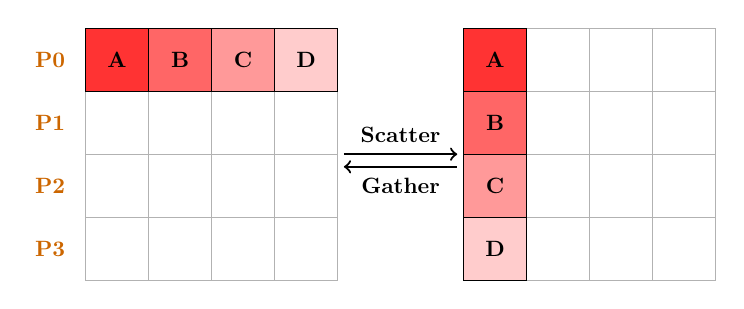
\begin{tikzpicture}[scale=0.8, every node/.style={scale=0.8}]
        %! --- Scatter / Gather ---
        % Process labels (left)
        \foreach \i/\p in {0/P0,1/P1,2/P2,3/P3} {
            \node[anchor=east] at (-0.2,3.5-\i) {\textcolor{orange!80!black}{\textbf{\p}}};
        }
        % Scatter left matrix
        \foreach \i in {0,...,3} {
            \foreach \j in {0,...,3} {
                \draw[gray!60] (0+\j,3-\i) rectangle (1+\j,4-\i);
            }
        }
        \node[fill=red!80,draw,minimum width=1cm,minimum height=1cm] at (0.5,3.5) {\textbf{A}};
        \node[fill=red!60,draw,minimum width=1cm,minimum height=1cm] at (1.5,3.5) {\textbf{B}};
        \node[fill=red!40,draw,minimum width=1cm,minimum height=1cm] at (2.5,3.5) {\textbf{C}};
        \node[fill=red!20,draw,minimum width=1cm,minimum height=1cm] at (3.5,3.5) {\textbf{D}};

        % Scatter right matrix
        \foreach \i in {0,...,3} {
            \foreach \j in {0,...,3} {
                \draw[gray!60] (6+\j,3-\i) rectangle (7+\j,4-\i);
            }
        }
        \node[fill=red!80,draw,minimum width=1cm,minimum height=1cm] at (6.5,3.5) {\textbf{A}};
        \node[fill=red!60,draw,minimum width=1cm,minimum height=1cm] at (6.5,2.5) {\textbf{B}};
        \node[fill=red!40,draw,minimum width=1cm,minimum height=1cm] at (6.5,1.5) {\textbf{C}};
        \node[fill=red!20,draw,minimum width=1cm,minimum height=1cm] at (6.5,0.5) {\textbf{D}};
        % Scatter arrow and label
        \draw[->,thick] (4.1,2) -- (5.9,2);
        \node at (5,2.3) {\textbf{Scatter}};
        
        % Gather arrow and label
        \draw[<-,thick] (4.1,1.8) -- (5.9,1.8);
        \node at (5,1.5) {\textbf{Gather}};
    \end{tikzpicture}
    % \caption{Scatter and Gather}
    \label{fig:scatter-gather}
\end{figure}

\item \textbf{Allgather:} The \plaintt{MPI\_Allgather} function is a collective operation that allows all processes in a communicator to exchange data with all other processes. It collects data from all processes and combines it at the root.

\begin{figure}[H]
    \centering
    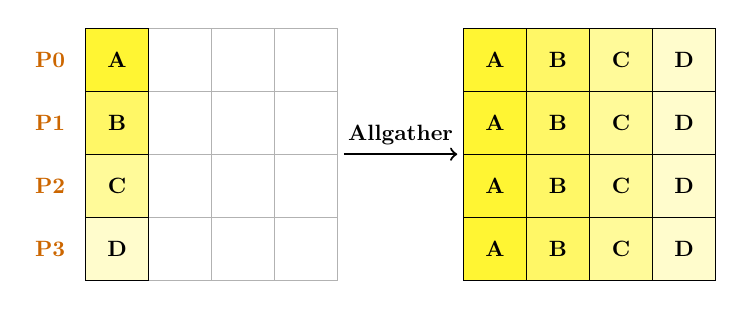
\begin{tikzpicture}[scale=0.8, every node/.style={scale=0.8}]
        % Process labels (left)
        \foreach \i/\p in {0/P0,1/P1,2/P2,3/P3} {
            \node[anchor=east] at (-0.2,3.5-\i) {\textcolor{orange!80!black}{\textbf{\p}}};
        }
        % Allgather left matrix
        \foreach \i in {0,...,3} {
            \foreach \j in {0,...,3} {
                \draw[gray!60] (0+\j,3-\i) rectangle (1+\j,4-\i);
            }
        }
        \node[fill=yellow!80,draw,minimum width=1cm,minimum height=1cm] at (0.5,3.5) {\textbf{A}};
        \node[fill=yellow!60,draw,minimum width=1cm,minimum height=1cm] at (0.5,2.5) {\textbf{B}};
        \node[fill=yellow!40,draw,minimum width=1cm,minimum height=1cm] at (0.5,1.5) {\textbf{C}};
        \node[fill=yellow!20,draw,minimum width=1cm,minimum height=1cm] at (0.5,0.5) {\textbf{D}};
        % Allgather right matrix
        \foreach \i in {0,...,3} {
            \foreach \j in {0,...,3} {
                \draw[gray!60] (6+\j,3-\i) rectangle (7+\j,4-\i);
            }
        }
        \foreach \j in {0,...,3} {
            \node[fill=yellow!80,draw,minimum width=1cm,minimum height=1cm] at (6.5,3.5-\j) {\textbf{A}};
            \node[fill=yellow!60,draw,minimum width=1cm,minimum height=1cm] at (7.5,3.5-\j) {\textbf{B}};
            \node[fill=yellow!40,draw,minimum width=1cm,minimum height=1cm] at (8.5,3.5-\j) {\textbf{C}};
            \node[fill=yellow!20,draw,minimum width=1cm,minimum height=1cm] at (9.5,3.5-\j) {\textbf{D}};
        }
        % Allgather arrow and label
        \draw[->,thick] (4.1,2) -- (5.9,2);
        \node at (5,2.3) {\textbf{Allgather}};
    \end{tikzpicture}
    % \caption{Allgather}
    \label{fig:allgather}
\end{figure}

\item \textbf{Alltoall:} The \plaintt{MPI\_Alltoall} function is a collective operation that allows all processes in a communicator to exchange data with every other process. Each process sends data to every other process, and each process receives data from every other process.

\begin{figure}[H]
    \centering
    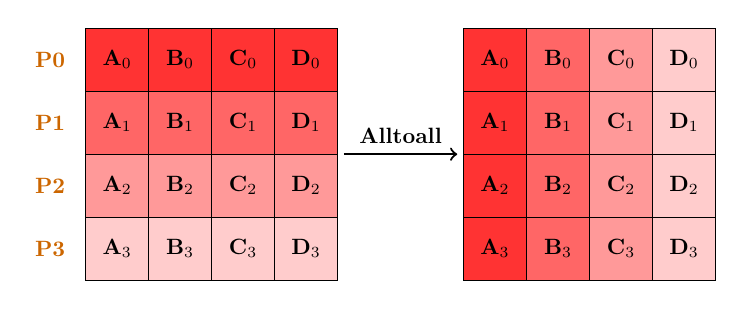
\begin{tikzpicture}[scale=0.8, every node/.style={scale=0.8}]
        % Process labels (left)
        \foreach \i/\p in {0/P0,1/P1,2/P2,3/P3} {
            \node[anchor=east] at (-0.2,3.5-\i) {\textcolor{orange!80!black}{\textbf{\p}}};
        }
        % Alltoall left matrix
        \foreach \i in {0,...,3} {
            \foreach \j in {0,...,3} {
                \draw[gray!60] (\j,3-\i) rectangle (1+\j,4-\i);
            }
        }
        % Fill left matrix
        \foreach \j/\lbl/\col in {0/A,1/B,2/C,3/D} {
            \node[fill=red!80,draw,minimum width=1cm,minimum height=1cm] at (0.5+\j,3.5) {\textbf{\lbl$_0$}};
            \node[fill=red!60,draw,minimum width=1cm,minimum height=1cm] at (0.5+\j,2.5) {\textbf{\lbl$_1$}};
            \node[fill=red!40,draw,minimum width=1cm,minimum height=1cm] at (0.5+\j,1.5) {\textbf{\lbl$_2$}};
            \node[fill=red!20,draw,minimum width=1cm,minimum height=1cm] at (0.5+\j,0.5) {\textbf{\lbl$_3$}};
        }
        % Alltoall right matrix
        \foreach \i in {0,...,3} {
            \foreach \j in {0,...,3} {
                \draw[gray!60] (6+\j,3-\i) rectangle (7+\j,4-\i);
            }
        }
        % Fill right matrix (transpose)
        \foreach \i/\lbl/\col in {0/A,1/B,2/C,3/D} {
            \node[fill=red!80,draw,minimum width=1cm,minimum height=1cm] at (6.5,3.5-\i) {\textbf{A$_\i$}};
            \node[fill=red!60,draw,minimum width=1cm,minimum height=1cm] at (7.5,3.5-\i) {\textbf{B$_\i$}};
            \node[fill=red!40,draw,minimum width=1cm,minimum height=1cm] at (8.5,3.5-\i) {\textbf{C$_\i$}};
            \node[fill=red!20,draw,minimum width=1cm,minimum height=1cm] at (9.5,3.5-\i) {\textbf{D$_\i$}};
        }
        % Alltoall arrow and label
        \draw[->,thick] (4.1,2) -- (5.9,2);
        \node at (5,2.3) {\textbf{Alltoall}};
    \end{tikzpicture}
    % \caption{Alltoall}
    \label{fig:alltoall}
\end{figure}
\end{itemize}